\section{Design}

\subsection{Overview}
\begin{figure*}[htbp]
	\centering
	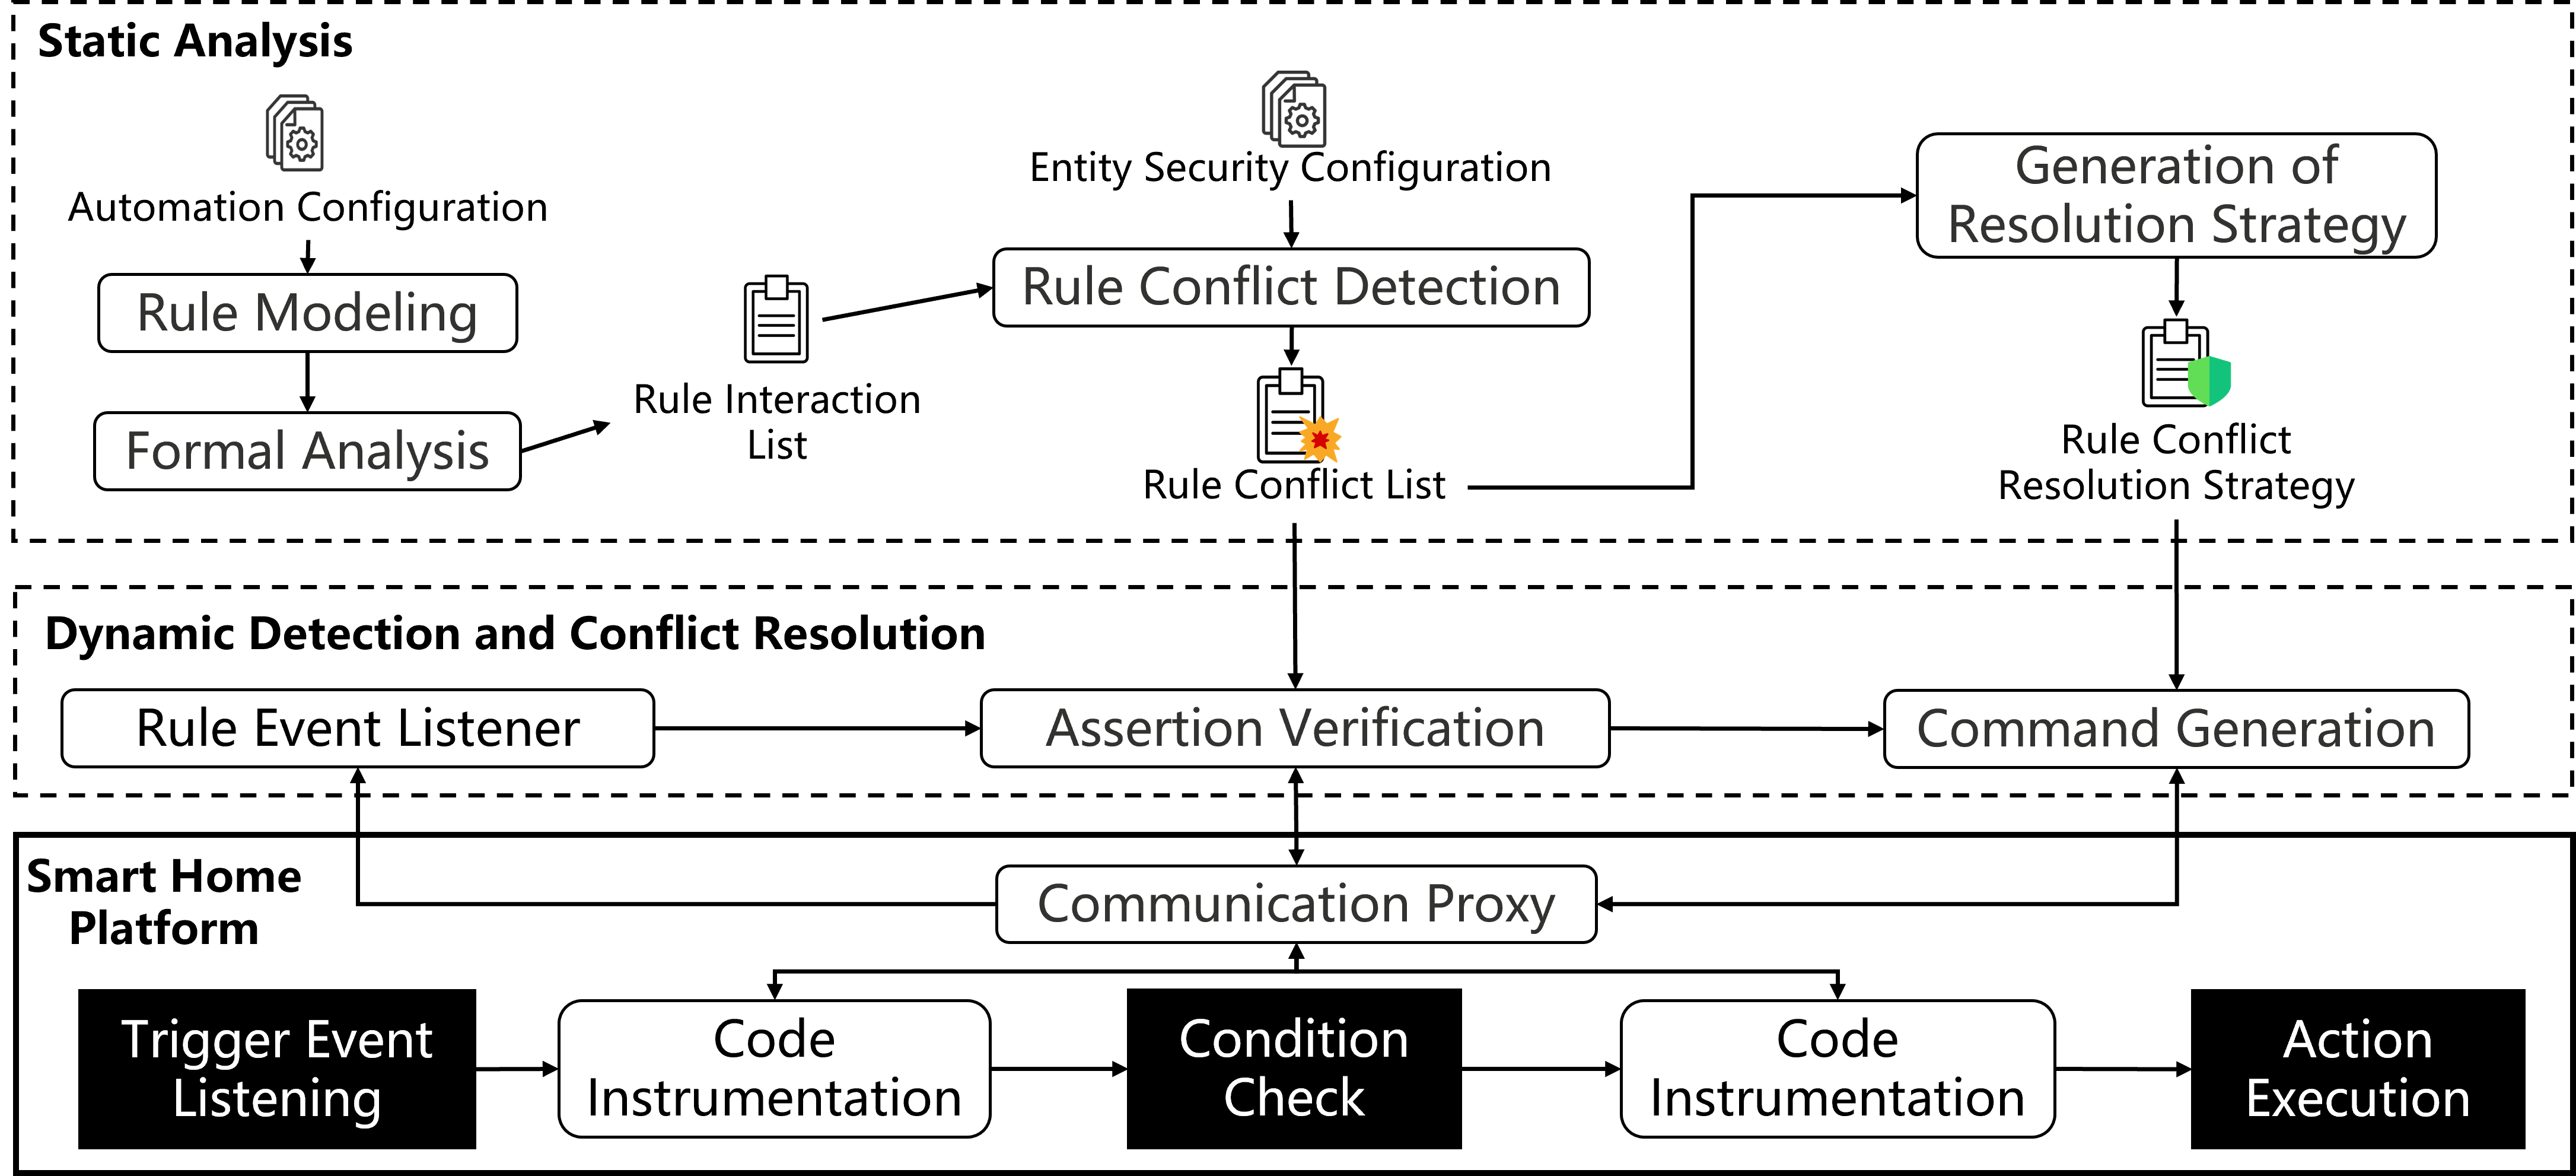
\includegraphics[width=\textwidth]{figure/overall_design.png}
	\caption{Overall Architecture of Our Approach}
	\label{overall_design}
\end{figure*}
% 本文设计了一个完整的系统,旨在通过静态与动态分析相结合的方式检测规则交互中存在的潜在规则冲突,并在冲突发生前自动执行定制化的冲突处理策略,避免实际冲突的发生。如图 Fig.\ref{overall_design} 所示,我们的方法主要包括两个阶段:1) 静态分析;2) 动态检测与冲突处理。
This paper presents a complete system designed to detect potential rule conflicts within rule interactions through a combination of static and dynamic analysis. The system automatically executes customized conflict resolution strategies before conflicts occur, preventing their actual manifestation. As illustrated in Fig.\ref{overall_design}, our approach primarily comprises two phases: 1) Static Analysis; 2) Dynamic Detection and Conflict Resolution.

% 静态分析阶段包含规则建模模块、形式化分析模块、静态规则冲突检测模块以及冲突处理策略生成模块。首先,对智能家居系统中的规则进行重新建模,以区分家庭环境中的不同区域。然后,形式化分析模块基于新的规则模型提取所有类型的规则交互,并生成相应的交互分析数据。用户的实体安全配置将应用于静态规则冲突检测模块,用于从规则交互集合中识别出真正的规则冲突。考虑到规则交互是否构成冲突具有主观性,系统提供用户配置界面,以自然语言的形式展示形式化分析模块提取的规则交互分析数据,辅助用户进行冲突判定。最后,冲突处理策略生成模块为每个已识别的规则冲突生成定制化的处理策略。
The static analysis phase includes a rule modeling module, a formal analysis module, a static rule conflict detection module, and a conflict resolution strategy generation module. Initially, the rules in the smart home system are remodeled to differentiate between zones within the environment. Subsequently, the formal analysis module extracts all types of rule interactions based on the new rule model and generates corresponding interaction analysis data. The user's entity safety configuration is then applied to the static rule conflict detection module, which identifies actual rule conflicts from the set of rule interactions. Recognizing the subjectivity inherent in defining a rule interaction as a conflict, the system presents the rule interaction data extracted by the formal analysis module to the user through a user configuration interface in natural language in order to facilitate the user determining rule conflicts. Finally, the conflict resolution strategy generation module generates customized resolution strategies for each identified rule conflict.

% 动态检测与冲突处理阶段包含规则事件监听模块、断言验证模块和命令生成模块。此外,智能家居系统(例如 Home Assistant)中的代码插桩模块将辅助完成动态规则冲突检测与预防。规则事件监听模块实时监听规则执行信息。当一条规则被触发,并在条件检查前后,该模块会将相关信息发送给断言验证模块。断言验证模块将基于历史规则执行事件、当前执行规则信息以及相关设备状态信息进行断言验证,判断规则冲突是否实际发生。若确认冲突即将发生,命令生成模块将根据静态分析阶段生成的冲突处理策略,生成相应的执行命令,并由代码插桩模块强制执行。
The dynamic detection and conflict resolution phase includes a rule event listener module, an assertion verification module, and a command generation module. Additionally, the code instrumentation module within the smart home system (e.g., Home Assistant) assists in dynamic rule conflict detection and prevention. The rule event listener module monitors the rule execution information in real time. When a rule is triggered, the listener module sends related information to the assertion verification module both before and after condition checking. Based on historical rule execution events, current rule information, and relevant device state information, the assertion verification module then performs assertion verification to determine whether a rule conflict has indeed occurred. If so, the command generation module will generate execution commands with the current rule conflict information about to occur and the rule conflict resolution strategy from static detection, which will be enforced by the code instrumentation module.

\subsection{Static Analysis}

\subsubsection{Rule Modeling}

%\begin{figure}[htbp]
%	\centering
%	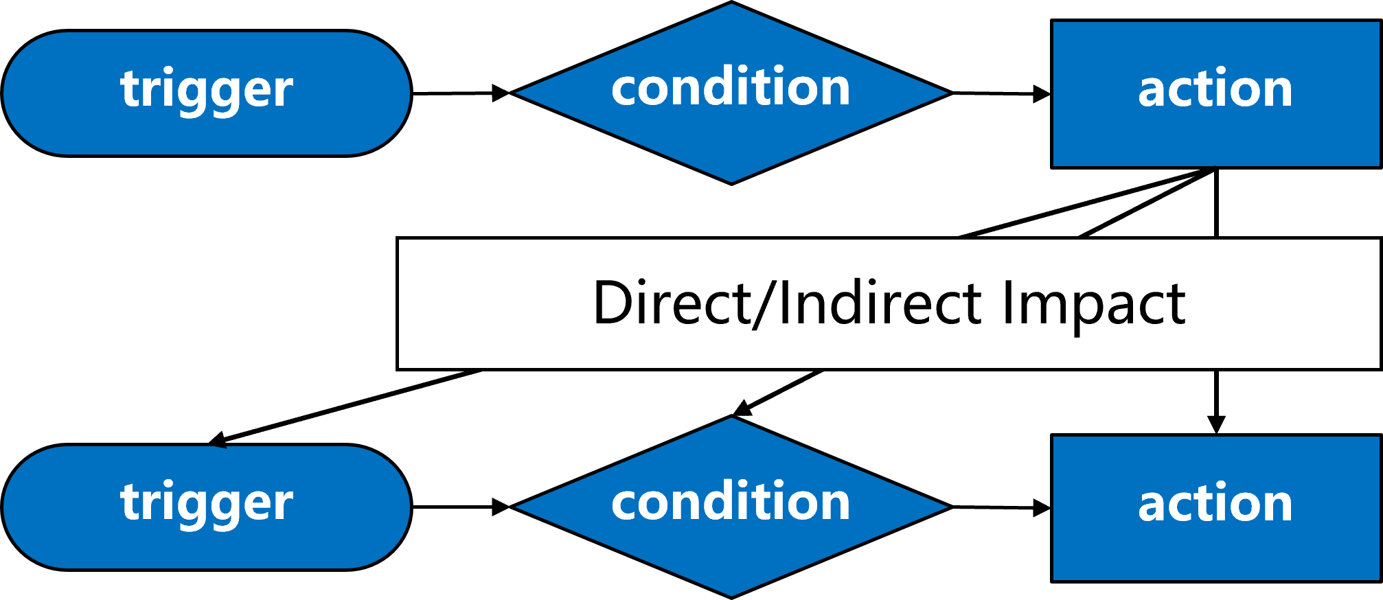
\includegraphics[width=0.4\textwidth]{figure/classification_observation.png}
%	\caption{Rule Interaction Pattern}
%	\label{classification_observation}
%\end{figure}

% 在介绍静态阶段之前,首先阐述本方案对规则交互与规则冲突的分类方法。基于之前的观察,我们将规则之间的交互归纳为:一条规则的执行结果对另一条规则的触发器、条件或动作产生直接或间接的影响。由此,我们将规则交互分为以下几类:触发器交互 (Trigger Interaction)、条件交互 (Condition Interaction)、动作交互 (Action Interaction)、间接触发器交互 (Indirect Trigger Interaction)、间接条件交互 (Indirect Condition Interaction) 和间接动作交互 (Indirect Action Interaction)。相应地,我们定义了六种规则冲突类型:触发器冲突 (Trigger Conflict)、条件冲突 (Condition Conflict)、动作冲突 (Action Conflict)、间接触发器冲突 (Indirect Trigger Conflict)、间接条件冲突 (Indirect Condition Conflict) 和间接动作冲突 (Indirect Action Conflict)。
Before formally introducing the static phase, it is necessary to the classification of rule interactions and rule conflicts for this approach. Based on previous observations Fig.\ref{classification_observation}, we summarize the interactions among rules as follows: the execution result of one rule can have direct and indirect impacts on the triggers, conditions, and actions of another rule. Thus, we can classify rule interactions as follows: Trigger Interaction, Condition Interaction, Action Interaction, Indirect Trigger Interaction, Indirect Condition Interaction, and Indirect Action Interaction. At the same time, six categories of rule conflicts can be identified: Trigger Conflict, Condition Conflict, Action Conflict, Indirect Trigger Conflict, Indirect Condition Conflict, and Indirect Action Conflict.

% 智能家居系统中的规则通常以静态文件形式存储,从中可以提取规则的触发器 (T)、条件 (C) 和动作 (A) 属性,并快速建模为 $\langle T,C,A \rangle$ 模型。然而,仅凭这些数据不足以检测不同家庭区域中侧面通道的影响,例如不同规则对卧室温度的影响所引发的交互,或者不同规则开启高功耗设备导致家庭用电功率升高,从而触发节电规则等。因此,需要引入新的属性 $E$。定义 $E=[e^1, e^2,\dots]$,$e^i=(area, channel, trend)$。其中,$area$ 表示间接通道的区域特征,如厨房、客厅或整个家庭等;$channel$ 表示侧面通道名称,如温度、湿度、光照强度等;$trend$ 表示该侧面影响的影响趋势,如升高、降低等。对于规则的触发器或条件,如果 $e$ 为 $\langle kitchen, temperature, increases\rangle$,则表示其他规则的执行结果可能导致厨房温度升高,从而使当前规则的触发器更易触发或条件更易满足。对于规则的动作,如果 $e$ 为 $\langle kitchen, temperature, increases\rangle$,则表示当前规则的执行可能导致厨房温度升高。属性 $E$ 基于用户真实的家庭情况和相关规则确定。例如,如果一个家庭中没有任何与 "湿度" 相关的规则,则无需将 $channel$ 设置为 "湿度"。由此,规则可以被重新建模为 $R=\langle T,C,A,E\rangle $ 或 $R=\langle T,C,A,E_T,E_C,E_A \rangle$ 形式,称为 TCAE 模型。
In smart home systems, rule configuration is usually stored as static files, from which the triggers, conditions, and action attributes of a rule can be extracted, and quickly modeled as a $\langle T,C,A \rangle$ model. However, the above data is insufficient to support the detection of the effects of side channels in different home areas within smart home systems. For example, rule interactions may be caused by different rules affecting the bedroom temperature, or by different rules turning on high-power devices, leading to an increase in the household's power consumption and subsequently triggering related rules to conserve electricity. Therefore, a new attribute $E$ needs to be introduced. $E$ is defined as$E=[e^1, e^2,\dots]$ and $e^i=(area, channel, trend)$, where $area$ indicates the spatial characteristics of the channel, such as the kitchen, living room, or the whole home; $channel$ indicates the name of the other channel which rules may impact each other, such as temperature, humidity, illuminance and so on; and $trend$ indicates the direction of the influence of the other channel, such as an increase and decrease. For the trigger/condition of a rule, if $e$ is $\langle kitchen, temperature, increases\rangle$, it means that if the execution results of other rules may lead to an increase in kitchen temperature, then the trigger/condition of the current rule is more likely to be met. For the action execution of a rule, if $e$ is $\langle kitchen, temperature, increases\rangle$, it means that the execution of the current rule may promote an increase in kitchen temperature. The attribute $E$ will be determined based on the user's actual home situation and the related rules. For example, if there are no rules concerning "humidity" in a home, then there is no need to set the $channel$ attribute of $e$ as "humidity". Thus, a rule can be re-modeled in the following form: $R=\langle T,C,A,E\rangle $ or $R=\langle T,C,A,E_T,E_C,E_A \rangle$ which called TCAE model.

\subsubsection{Formal Analysis}

\begin{table*}[htbp]
	\begin{center}
		\caption{Formal Analysis Expression}
		\label{Formal_Analysis_Expression}
		\begin{adjustbox}{width=0.95\textwidth}
			\begin{tabular}[width=0.95\textwidth]{c|c} 
				\hline
				\textbf{Classification} & \textbf{Expression}\\
				\hline
				\text{Trigger Interaction} & $(\exists a_{1}\in A_{1})\wedge(a_{1}\rightarrow T_{2})$ \\
				\hline
				\text{Condition Interaction} & $\left((A_{1}\nrightarrow C_{2})\wedge\left((T_{1}\neq T_{2})\wedge(R_{1}\neq R_{2})\right)\right)\vee\left((A_{1}\to\mathcal{C}_{2})\wedge\left((T_{1}\neq T_{2})\wedge(R_{1}\neq R_{2})\right)\right)$ \\
				\hline
				\text{Action Interaction} & $(\exists a_{1}\in A_{1})\wedge(\exists a_{2}\in A_{2})\wedge(a_{1}\perp a_{2})$ \\
				\hline
				\text{Indirect Trigger Interaction} & $(\exists a_{1}\in A_{1})\wedge\left(E_{a_{1}}=E_{T_{1}}\right)$ \\
				\hline
				\text{Indirect Condition Interaction} & $\left(\left(E_{A_{1}}\perp E_{C_{2}}\right)\vee\left(E_{A_{1}}=E_{C_{2}}\right)\right)\wedge\left(R_{1}\neq R_{2}\right)$ \\
				\hline
				\text{Indirect Action Interaction} & $(\exists a_{1}\in A_{1})\wedge(\exists a_{2}\in A_{2})\wedge\left(D_{a_{1}}\neq D_{a_{2}}\right)\wedge\left(E_{a_{1}}\perp E_{a_{2}}\right)$ \\
				\hline
			\end{tabular}
		\end{adjustbox}
	\end{center}
\end{table*}

% 基于 TCA 模型进行规则冲突分类,假设规则 $R_1=\langle T_1,C_1,A_1,E_{T_1},E_{C_1},E_{A_1} \rangle$ 和 𝑅₂=(𝑇₂, 𝐶₂, 𝐴₂, 𝐸(𝑇₂), 𝐸(𝐶₂), 𝐸(𝐴₂)) 表示在同一系统中设置的两条规则。其中,T、C、A 和 E 分别表示对应的属性。本文使用 $\rightarrow$ 表示促使触发器触发或条件满足,$\nrightarrow$ 表示禁止条件满足。对于 channel 属性,$\bot$ 表示两个 channel 属性具有相同的 $area$ 和 $channel$,但 $trend$ 相反(例如,厨房温度升高与厨房温度降低)。此外,$\bot$ 也表示两个动作相互冲突(例如,开启空调与关闭空调)。"=" 表示两个 channel 属性具有相同的 $area$、$channel$ 和 $trend$,或者两个触发器或条件相同。
According to the TCA model for rule conflict classification, let rule $R_1=\langle T_1,C_1,A_1,E_{T_1},E_{C_1},E_{A_1} \rangle$ and rule  $R_2=\langle T_2,C_2,A_2,E_{T_2},E_{C_2},E_{A_2} \rangle$ be to represent two rules set in the same system, where T, C, A, and E respectively represent the corresponding attribute. This paper uses $\rightarrow$ to indicate that a trigger is activated or a condition is met, and $\nrightarrow$ to indicate that a condition is prohibited.$\bot$ denotes that the two channel attributes have the same area and channel but opposite trends (for example, rising kitchen temperature versus falling kitchen temperature), or it indicates that two actions are in conflict (such as turning on the air conditioner versus turning it off), while "=" indicates that the two channel attributes have the same area, channel, and trend, or that there are two identical triggers or conditions.

% 形式化分析模块遍历每个规则模型,并进行表达式验证。若表达式成立,则表示两条规则满足对应的规则交互类型。规则冲突是规则交互的特例,因此,该表达式仅用于筛选存在交互的规则,而要判断规则交互是否构成实际的规则冲突,还需要进一步的检测。具体的表达式如 Table.\ref{Formal_Analysis_Expression} 所示。由此,形式化分析模块能够分析得到具体的规则交互列表,其中包含了所有规则交互及其交互模式信息。
The formal analysis module will traverse each rule model and then expression validation. If an expression is satisfied, it indicates that the two rules meet the corresponding rule interaction classification. Rule conflict is a special case of rule interaction, and that expression can only filter out interacting rules. further detection is required to determine whether a rule interaction constitutes a rule conflict.The formal analysis module can analyze and obtain a specific list of rule interactions, which includes all rule interactions and interaction pattern information.

\subsubsection{Rule Conflict Detection and Resolution Strategy Generation}
% 实体安全配置是安全敏感设备实体的安全状态集合,用于表示智能家居系统中发生冲突时应优先保持的状态。例如,门应保持 "关闭" 状态,消防喷淋头应保持 "开启" 状态。规则冲突检测模块对规则交互列表中的每个元素进行实体安全检查,以确定规则交互是否违反实体安全状态,从而引发潜在的规则冲突。
Entity safety configuration is a set of safety states for a security-sensitive device entity, used to indicate the preferred state to maintain when a conflict occurs in a smart home system—for example, a door should be "closed" and a fire sprinkler should be "on." The rule conflict detection module performs an entity safety on all elements in the rule interaction list to determine whether a rule interaction violates the entity safety state, potentially causing a rule conflict.

% 具体的检查方法如下:对于包含两条规则的规则交互,需要关注交互完成后是否违反实体安全配置的要求。为此,为每条规则设定一个安全值参数 $sf$。若规则的执行结果更符合实体安全状态配置,则 $sf$ 值越高,反之越低。$sf$ 值通过遍历所有实体安全配置,采用线性函数计算。例如,若规则的执行结果是关闭门,这符合实体 "门" 的安全状态 "关闭",则该规则的 $sf$ 值在原有基础上加一,反之则减一。默认值为零。
The specific inspection method is as follows: a rule interaction includes two rules, and attention should be paid to whether the entity safety configuration requirements are violated after this rule interaction is completed. Therefore, each rule sets a safety value parameter, $sf$. If the execution result of a rule is more inclined to meet the entity safety configuration, the $sf$ value is higher; otherwise, it is lower. The specific $sf$ value can be calculated using a linear function by traversing all the entity safety configurations. For example, if the execution result of a rule is closing a door, which is more in line with the entity safety state "closed" for the entity "door", then the rule's $sf$ is increased by one from the original value, Otherwise, it is decreased by one, with the default value being zero.

% 针对不同类型的规则交互,规则冲突的判定方法有所不同:
% \begin{itemize}
	% 	\item 对于触发器交互和间接触发器交互,关注第二条规则的安全值 $sf$ 是否大于零。若小于零,则判定为规则冲突。
	% 	\item 对于条件交互和间接条件交互,若第一个规则禁止了第二个规则的条件,且第二个规则的 $sf$ 大于零,则判定为规则冲突;反之,若第一个规则使得第二个规则的条件得以满足,且第二个规则的 $sf$ 小于零,也判定为规则冲突。这表明前一条规则的影响导致后一条更符合实体安全状态的规则未被执行,或导致后一条与实体安全状态相违背的规则被执行。
	% 	\item 对于动作交互和间接动作交互,若其中包含的两条规则的安全值之一不为零,则判定为规则冲突。需要注意的是,即使两条规则的安全值都大于零,仍可能判定为规则冲突,因为此类交互中的两条规则的执行结果是相互矛盾的,通常只需执行其中一条规则。
	% \end{itemize}
For different rule interactions, the method for determining rule conflicts varies. 
\begin{itemize}
	\item For Trigger Interaction and Indirect Trigger Interaction, the focus is on whether the safety value $sf$ of the second rule is greater than zero; if it is less than zero, then it is determined to be a rule conflict.
	\item For Condition Interaction and Indirect Condition Interaction, if the first rule in a rule interaction prohibits the condition of the second rule while the second rule’s $sf$ is greater than zero, it is determined to be a rule conflict; or if the first rule satisfies the condition of the second rule while the second rule’s $sf$ is less than zero, it is determined to be a rule conflict. This indicates that due to the influence of the preceding rule, either the rule that is more inclined to the entity safety state was not executed for the latter rule, or the rule that contradicts the entity safety state was executed.
	\item For Action Interaction and Indirect Action Interaction, if either of the two rules has a non-zero safety value, it is determined to be a rule conflict. In this case, it should be noted that if both rules have safety values greater than zero, it will also be deemed a rule conflict, because in the determination of this type of rule interaction, the execution results of the two rules are contradictory, and typically only one rule needs to be executed.
\end{itemize}

% 由此,可以为每种规则冲突设定多种处理策略。具体的冲突处理策略可根据 Table.\ref{Resolution_Policy_Decision} 进行选择。
Based on this, multiple resolution strategies can be set for each rule. The specific conflict resolution strategy can be selected according to Table.\ref{Resolution_Policy_Decision}.

\begin{table*}[htbp]
	\begin{center}
		\caption{Resolution Policy Decision (Need modification)}
		\label{Resolution_Policy_Decision}
		\begin{adjustbox}{width=0.95\textwidth}
		\begin{tabular}{c|c|c}
			\hline
			\textbf{Classification} & \textbf{Decision} & \textbf{Options} \\
			\hline
			\multirow{3}{*}{\makecell{\textbf{Trigger Conflict} \\ \textbf{Indirect Trigger Conflict}}} 
			& $(sf_2 = 0)\vee(sf_2>0 \wedge sf_1\geq 0)$ & Not rule conflict \\
			\cline{2-3}
			& $sf_1 < 0 \land sf_2 \geq 0$ & Only execute $R_2$ \\
			\cline{2-3}
			& $sf_2 < 0$ & Cancel execution of $R_2$ \\
			\hline
			\multirow{3}{*}{\makecell{\textbf{Condition Conflict} \\ \textbf{Indirect Condition Conflict}}} 
			& $(A_{1}\rightarrow C_{2}\wedge sf_{2}>0)\vee(A_{1}\nrightarrow C_{2}\wedge sf_{2}<0)$ & Not rule conflict \\
			\cline{2-3}
			& $A_{1}\rightarrow C_{2}\wedge sf_{2}>0$ & Do not execute $R_2$\\
			\cline{2-3}
			& $A_{1}\nrightarrow C_{2}\wedge sf_{2}<0$ & Execute $R_2$ \\
			\hline
			\multirow{6}{*}{\makecell{\textbf{Action Conflict} \\ \textbf{Indirect Action Conflict}}} 
			& $sf_1 = 0 \land sf_2 = 0$ & Not rule conflict \\
			\cline{2-3}
			& $sf_1 > 0 \land sf_2 < 0$ & Only execute $R_1$ \\
			\cline{2-3}
			& $sf_1 < 0 \land sf_2 > 0$ & Only execute $R_2$ \\
			\cline{2-3}
			& $sf_1 > 0 \land sf_2 > 0 \land sf_1 > sf_2$ & Both rules are executed, but ended with $R_1$ \\
			\cline{2-3}
			& $sf_1 > 0 \land sf_2 > 0 \land sf_1 < sf_2$ & Both rules are executed, but ended with $R_2$ \\
			\cline{2-3}
			& $sf_1 < 0 \land sf_2 < 0$ & Neither rule will be executed \\
			\hline
		\end{tabular}
		\end{adjustbox}
	\end{center}
\end{table*}

\subsection{Dynamic Detection and Conflict Resolution}
\subsubsection{Assertion Verification}
%静态检测部分全部离线运行,Dynamic detection and Conflict resolution部分将会以静态检测的输出结果作为基础,例如Rule Conflict List和Rule Conflict Resolution Strategy,对规则冲突进行实时监测与预防。Dynamic detection and Conflict resolution的Rule Event Listener module和Command Generation module主要依赖代码插装,实现对规则事件的监听与实现在冲突事件发生前对设备的默认操作拦截与冲突处理策略执行,因此以下部分重点介绍Assertion Verification module
The static detection part runs entirely offline, while the dynamic detection and conflict resolution part will be based on the output of the static detection, such as the rule conflict list and rule conflict resolution strategy, to monitor and prevent rule conflicts in real-time. The rule event listener module and command generation module of dynamic detection and conflict resolution mainly rely on code instrumentation to listen to rule events and implement the interception of the device's default operations and the execution of conflict resolution strategies before conflict events occur. Therefore, the following part focuses on the assertion verification module.

%,在智能家居系统运行时,所有规则事件将被实时监听。当一条规则被触发后,在其条件检查阶段前后都会进行断言检测,以判断当前系统是否即将发生规则冲突。断言检测过程中的所有信息都将通过代码插桩模块获取,包括当前执行规则的信息、过去执行规则的信息,以及相关实体设备的实时状态与历史状态变化信息等。
When the smart home system is running, rule events will be monitored in real-time. When a rule is triggered, assertion verification will be performed before and after the condition checking phase to determine whether a rule conflict is imminent. All information during the assertion verification process will be collected through the code instrumentation module, including the information of the currently executing rule, the information of the previously executed rule, the real-time status of related entities, and past state change information.

% 断言检测主要包含以下函数:
Assertion detection mainly includes the following functions:

\begin{itemize}
	\item $obs()$: Observing the occurrence of an event (including the triggering of the trigger $obs(T)$,the passing of a condition check $obs(C)$, the failing of a condition check $obs(\neg C)$ and the execution of an action $obs(A)$
	\item $intime(X,Y,\delta)$: the time interval between events $X$ and $Y$ is less than $\delta$, with $\delta$ defaulting to 0.1 seconds
\end{itemize}

% 由此,针对不同类型的规则冲突,存在对应的断言检测方法,如 Table.\ref{Assertion_Verification} 所示。
Accordingly, for different types of rule conflicts, there are corresponding assertion verification methods, as shown in Table.\ref{Assertion_Verification}.

% 例如存在两条规则$R_1$和$R_2$在静态检测中属于Trigger Conoflict类型的规则冲突,断言检测过程如下:(1)第一步,分别观察到$T_1$,$C_1$和$A_1$的发生,表明表明规则$R_1$触发并通过条件检测后成功执行预期动作;(2)第二步,分别观察到$T_2$和$C_2$的发生,表明规则$R_2$触发并通过了条件检测,平台及将执行$R_2$的默认动作;(3)观察到$A_1$和$T_2$两个事件的发生的时间间隔很短,时间间隔小于阈值$delta$。三个步骤全部为真则可以认为是规则$R_1$的执行导致了规则$R_2$被触发并即将执行,为了防止真实世界中的巧合发生,即避免是因为其他现实原因规则$R_1$与规则$R_2$在符合用户预期条件下分别短时间内出发并执行而导致误判,这里的$delta$通常设置很小的值,如0.1秒甚至0.01秒。不必担心因为系统执行时的必然时间损耗导致阈值$delta$偏小而引起规则冲突没有被监测出,因为系统中的时间损耗极低,通常为毫秒级别。
For example, if there are two rules, $R_1$ and $R_2$, that belong to the Trigger Conflict type of rule conflict in static detection, the assertion verification process is as follows: (1) First, observe the occurrence of $T_1$, $C_1$, and $A_1$, indicating that rule $R_1$ is triggered, passes the condition check, and successfully executes the expected action; (2) Second, observe the occurrence of $T_2$ and $C_2$, indicating that rule $R_2$ is triggered and passes the condition check, and the platform is about to execute the default action of $R_2$; (3) Observe that the time interval between the occurrence of events $A_1$ and $T_2$ is very short, less than the threshold $delta$. If all three steps are true, it can be considered that the execution of rule $R_1$ caused rule $R_2$ to be triggered and about to be executed. To prevent coincidences in the real world, i.e., to avoid misjudgments caused by other real-world reasons where rule $R_1$ and rule $R_2$ are triggered and executed in a short time under conditions that meet user expectations, the $delta$ here is usually set to a very small value, such as 0.1 seconds or even 0.01 seconds. There is no need to worry that the inevitable time loss during system execution will cause the threshold $delta$ to be too small and cause rule conflicts to not be detected, because the time loss in the system is extremely low, usually on the order of milliseconds.

\begin{table}[t]
	\caption{Assertion Verification Expression}
	\label{Assertion_Verification}
	\begin{adjustbox}{width=0.5\textwidth}
		\begin{tabular}[width=1\textwidth]{c|c|c}
			\hline
			\multicolumn{2}{c|}{\textbf{Classification}} & \textbf{Expression}\\
			\hline
			
			\multicolumn{2}{c|}{\textbf{Trigger Conflict}} &
			\makecell{
				$obs(T_1), obs(C_1), obs(A_1)$ \\
				$obs(T_2), obs(C_2)$ \\
				$intime(A_1, T_2, delta)$}\\
			\hline
			
			\multirow{2}{*}{\textbf{Condition Conflict}} & Make Conditions Forbidden &
			\makecell{$obs(C_2)$ \\
				$obs(T_1), obs(C_1), obs(A_1)$ \\
				$obs(\neg C_2)$ \\
				$intime(A_1, \neg C_2, delta)$} \\
			\cline{2-3}
			& Make Conditions Satisfied &
			\makecell{$obs(\neg C_2)$ \\
				$obs(T_1), obs(C_1), obs(A_1)$ \\
				$obs(C_2)$\\
				$intime(A_1, C_2, delta)$ }\\
			\hline
			
			\multicolumn{2}{c|}{\textbf{Action Conflict}} &
			\makecell{
				$obs(T_1), obs(C_1), obs(A_1)$ 
				\\ $obs(T_2), obs(C_2)$}\\
			\hline
			
			\multicolumn{2}{c|}{\textbf{Indirect Trigger Conflict}} &
			\makecell{$obs(T_1), obs(C_1), obs(A_1)$ \\
				$obs(T_2), obs(C_2)$} \\
			\hline
			
			\multirow{2}{*}{\textbf{Indirect Condition Conflict}} & Make Conditions Forbidden &
			\makecell{$obs(C_2)$ \\
				$obs(T_1), obs(C_1), obs(A_1)$ \\
				$obs(\neg C_2)$  \\
				$intime(A_1, \neg C_2, delta)$ }\\
			\cline{2-3}
			& Make Conditions Satisfied &
			\makecell{$obs(\neg C_2)$ \\
				$obs(T_1), obs(C_1), obs(A_1)$ \\
				$obs(C_2)$ \\
				$intime(A_1,  C_2, delta)$ }\\
			\hline
			
			\multicolumn{2}{c|}{\textbf{Indirect Action Conflict}}&
			\makecell{$obs(T_1), obs(C_1), obs(A_1)$ \\
				$obs(T_2), obs(C_2)$} \\
			\hline
			
		\end{tabular}
	\end{adjustbox}
\end{table}

% 当断言检测结果表明当前即将发生某一类型的规则冲突时,系统立即执行相应的冲突处理策略。具体执行方式为:基于静态检测中的Rule Conflict Resolution Strategy,系统检索规则冲突对应的冲突处理策略,生成具体的执行命令,通过Communication Proxy module交付给代码插桩模块。代码插桩模块拦截原有的规则触发执行逻辑(即触发、条件检测与动作执行),并强制执行对应的冲突处理策略对应的动作,从而实现在规则冲真实发生前,检测到规则冲突并进行冲突处理。
When the assertion verification result indicates that a certain type of rule conflict is about to occur, the system immediately executes the corresponding conflict resolution strategy. The specific execution method is as follows: Based on the Rule Conflict Resolution Strategy in static detection, the system retrieves the conflict resolution strategy corresponding to the rule conflict, generates specific execution commands, and delivers them to the code instrumentation module through the Communication Proxy module. The code instrumentation module intercepts the original rule trigger execution logic (i.e., trigger, condition detection, and action execution) and forcibly executes the action corresponding to the corresponding conflict resolution strategy, thereby achieving the detection of rule conflicts and conflict resolution before the rule actually occurs.
\subsubsection{Code Instrumentation}
%代码插装模块在Dynamic Detection and Conflict Resolution中起到了至关重要的作用。
Code instrumentation modules play a crucial role in Dynamic Detection and Conflict Resolution.

%在规则冲突的动态检测过程中,代码插装模块与规则事件监听模块交互,在规则的条件检查前后进行监听,保证了两种特殊情况:(1)一条原本条件不通过的规则,因为规则交互导致条件通过,并被成功触发;(2)原本条件检测通过的规则,因为规则交互导致条件不通过,并被成功触发。代码插装模块与断言检测模块交互,其核心功能包含两条通信函数:(1)get_entity_state用于获取实体状态,从而读取设备与规则的当前状态与历史状态变化信息,从而帮助断言检测模块获取所有验证需要的信息。(2)time_now用户获取系统当前事件,避免因为系统时间与实际时间偏差导致检测与处理错误。
In the dynamic detection of rule conflicts, the code instrumentation module interacts with the rule event listening module to listen before and after the condition check of the rules, ensuring two special cases: (1) a rule that originally did not pass the condition can pass the condition due to rule interaction and be successfully triggered; (2) a rule that originally passed the condition check can fail the condition due to rule interaction and be successfully triggered. The code instrumentation module interacts with the assertion verification module, and its core functions include two communication functions: (1) \texttt{get\_entity\_state} is used to obtain the entity state, so as to read the current state and historical state change information of the device and the rule, so as to help the assertion verification module obtain all the information needed for verification. (2) \texttt{time\_now} is used to obtain the current event of the system, so as to avoid detection and processing errors caused by the deviation between the system time and the actual time.

%在规则冲突的处理过程中,代码插装模块与规则命令生成模块交互,在规则的条件检查前后进行插入,保证了两种特殊情况:(1)一条原本条件不通过的规则,因为规则交互导致条件通过,并被成功触发;(2)原本条件检测通过的规则,因为规则交互导致条件不通过,并被成功触发。其核心功能为拦截当前规则的执行动作并执行从命令生成模块生成的指令,如强制执行当前条件不通过的规则,强制执行某条规则的执行动作等等。
In the process of handling rule conflicts, the code instrumentation module interacts with the rule command generation module to insert code before and after the rule's condition check. This ensures two special cases: (1) a rule that originally failed the condition check can pass the condition and be successfully triggered due to rule interaction; (2) a rule that originally passed the condition check can fail the condition and still be successfully triggered due to rule interaction. Its core function is to intercept the execution action of the current rule and execute the instructions generated from the command generation module, such as forcibly executing the current rule with a failed condition, forcibly executing the execution action of a certain rule, and so on.